\subsection{Adding a New Aspect to Your Project}
Create a new Class and name it \code{World}. Edit the buffer so it looks as follows and then save it:\\\\
\begin{verbatim}
Hier kommt dann der Code hin, der in aspect.png abgelegt ist.
private RootNode buildTreeModel(String path)
	{
		try {
      //TODO BUG: bei Zwei ge�ffneten Projekten wird nicht die Auswahl 
      //          des aktuellen Projekts genommen, sondern das, was als
			//          letztes gebuildet wurde!!!
			ProjectProperties projectProperties = new ProjectProperties(Builder.getLastBuildTarget());
			log.debug(projectProperties.getProjectLocation()+projectProperties.getOutputPath());
			globalPathForInformationAdapter = projectProperties.getProjectLocation()+projectProperties.getOutputPath();
		} catch(Exception e)
		{
		
		}
\end{verbatim}
%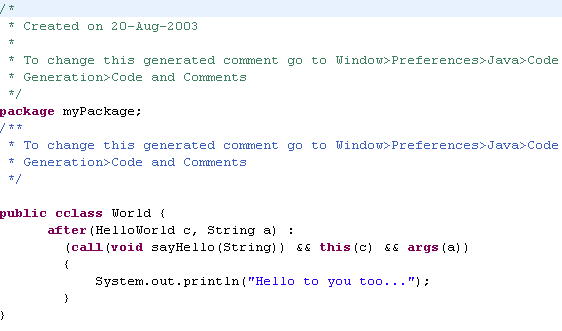
\includegraphics[width=0.80\textwidth]{images/aspect.png}\\

Make a clean Build of the project, and the outline view populates. Expand the \code{after()} node.\\\\
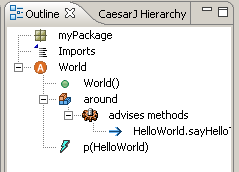
\includegraphics[width=0.5\textwidth]{images/aspect2.png}\newpage

You can see that this advice is affecting the HelloWorld.sayHello() method. Clicking on the \code{HelloWorld.sayHello()} node in the outline takes you to the declaration of HelloWorld.sayHello().

Notice the \code{advice annotation} in the editor buffer (highlighted) and that the \code{sayHello} method in the outline view shows that it is advised by the World aspect.\\\\
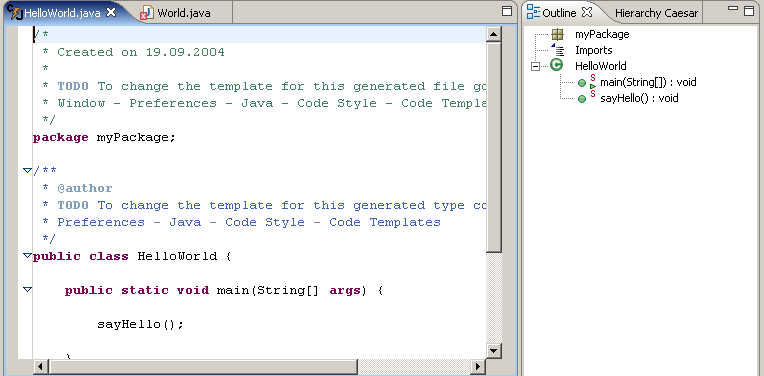
\includegraphics[width=0.95\textwidth]{images/aspect3.png}\\\\

Selecting the \code{World.after()} node in the outline view takes you back to the advice declaration. Right-clicking on the advice annotation brings up a context menu that also allows you to navigate to the advice.\\\\
\textbf{TODO BILD FEHLT KONNTE ICH NICHT SCREENSHOOT MACHEN  Weil es nicht geht EDITOR mit ADVICE CONTEXT}

